\documentclass[journal,12pt,twocolumn]{IEEEtran}
%
\usepackage{setspace}
\usepackage{gensymb}
\usepackage{xcolor}
\usepackage{caption}
\usepackage{circuitikz}
%\usepackage{subcaption}
%\doublespacing
\singlespacing
\usepackage{float}
%\usepackage{graphicx}
%\usepackage{amssymb}
%\usepackage{relsize}
\usepackage[cmex10]{amsmath}
\usepackage{mathtools}
%\usepackage{amsthm}
%\interdisplaylinepenalty=2500
%\savesymbol{iint}
%\usepackage{txfonts}
%\restoresymbol{TXF}{iint}
%\usepackage{wasysym}
\usepackage{hyperref}
\usepackage{amsthm}
\usepackage{mathrsfs}
\usepackage{txfonts}
\usepackage{stfloats}
\usepackage{cite}
\usepackage{cases}
\usepackage{subfig}
%\usepackage{xtab}
\usepackage{longtable}
\usepackage{multirow}
%\usepackage{algorithm}
%\usepackage{algpseudocode}
%\usepackage{enumerate}
\usepackage{enumitem}
\usepackage{mathtools}
%\usepackage{iithtlc}
%\usepackage[framemethod=tikz]{mdframed}
\usepackage{listings}
\let\vec\mathbf


%\usepackage{stmaryrd}


%\usepackage{wasysym}
%\newcounter{MYtempeqncnt}
\DeclareMathOperator*{\Res}{Res}
%\renewcommand{\baselinestretch}{2}
\renewcommand\thesection{\arabic{section}}
\renewcommand\thesubsection{\thesection.\arabic{subsection}}
\renewcommand\thesubsubsection{\thesubsection.\arabic{subsubsection}}

\renewcommand\thesectiondis{\arabic{section}}
\renewcommand\thesubsectiondis{\thesectiondis.\arabic{subsection}}
\renewcommand\thesubsubsectiondis{\thesubsectiondis.\arabic{subsubsection}}

%\renewcommand{\labelenumi}{\textbf{\theenumi}}
%\renewcommand{\theenumi}{P.\arabic{enumi}}

% correct bad hyphenation here
\hyphenation{op-tical net-works semi-conduc-tor}

\lstset{
language=Python,
frame=single, 
breaklines=true,
columns=fullflexible
}



\begin{document}
%

\theoremstyle{definition}
\newtheorem{theorem}{Theorem}[section]
\newtheorem{problem}{Problem}
\newtheorem{proposition}{Proposition}[section]
\newtheorem{lemma}{Lemma}[section]
\newtheorem{corollary}[theorem]{Corollary}
\newtheorem{example}{Example}[section]
\newtheorem{definition}{Definition}[section]
%\newtheorem{algorithm}{Algorithm}[section]
%\newtheorem{cor}{Corollary}
\newcommand{\BEQA}{\begin{eqnarray}}
\newcommand{\EEQA}{\end{eqnarray}}
\newcommand{\define}{\stackrel{\triangle}{=}}
\newcommand{\myvec}[1]{\ensuremath{\begin{pmatrix}#1\end{pmatrix}}}
\newcommand{\mydet}[1]{\ensuremath{\begin{vmatrix}#1\end{vmatrix}}}

\bibliographystyle{IEEEtran}
%\bibliographystyle{ieeetr}

\providecommand{\nCr}[2]{\,^{#1}C_{#2}} % nCr
\providecommand{\nPr}[2]{\,^{#1}P_{#2}} % nPr
\providecommand{\mbf}{\mathbf}
\providecommand{\pr}[1]{\ensuremath{\Pr\left(#1\right)}}
\providecommand{\qfunc}[1]{\ensuremath{Q\left(#1\right)}}
\providecommand{\sbrak}[1]{\ensuremath{{}\left[#1\right]}}
\providecommand{\lsbrak}[1]{\ensuremath{{}\left[#1\right.}}
\providecommand{\rsbrak}[1]{\ensuremath{{}\left.#1\right]}}
\providecommand{\brak}[1]{\ensuremath{\left(#1\right)}}
\providecommand{\lbrak}[1]{\ensuremath{\left(#1\right.}}
\providecommand{\rbrak}[1]{\ensuremath{\left.#1\right)}}
\providecommand{\cbrak}[1]{\ensuremath{\left\{#1\right\}}}
\providecommand{\lcbrak}[1]{\ensuremath{\left\{#1\right.}}
\providecommand{\rcbrak}[1]{\ensuremath{\left.#1\right\}}}
\theoremstyle{remark}
\newtheorem{rem}{Remark}
\newcommand{\sgn}{\mathop{\mathrm{sgn}}}
\providecommand{\abs}[1]{\left\vert#1\right\vert}
\providecommand{\res}[1]{\Res\displaylimits_{#1}} 
\providecommand{\norm}[1]{\lVert#1\rVert}
\providecommand{\mtx}[1]{\mathbf{#1}}
\providecommand{\mean}[1]{E\left[ #1 \right]}
\providecommand{\fourier}{\overset{\mathcal{F}}{ \rightleftharpoons}}
\providecommand{\ztrans}{\overset{\mathcal{Z}}{ \rightleftharpoons}}

%\providecommand{\hilbert}{\overset{\mathcal{H}}{ \rightleftharpoons}}
\providecommand{\system}{\overset{\mathcal{H}}{ \longleftrightarrow}}
	%\newcommand{\solution}[2]{\textbf{Solution:}{#1}}
\newcommand{\solution}{\noindent \textbf{Solution: }}
\providecommand{\dec}[2]{\ensuremath{\overset{#1}{\underset{#2}{\gtrless}}}}
\numberwithin{equation}{section}
%\numberwithin{equation}{subsection}
%\numberwithin{problem}{subsection}
%\numberwithin{definition}{subsection}
\makeatletter
\@addtoreset{figure}{problem}
\makeatother

\let\StandardTheFigure\thefigure
%\renewcommand{\thefigure}{\theproblem.\arabic{figure}}
\renewcommand{\thefigure}{\theproblem}


\numberwithin{figure}{subsection}

\def\putbox#1#2#3{\makebox[0in][l]{\makebox[#1][l]{}\raisebox{\baselineskip}[0in][0in]{\raisebox{#2}[0in][0in]{#3}}}}
     \def\rightbox#1{\makebox[0in][r]{#1}}
     \def\centbox#1{\makebox[0in]{#1}}
     \def\topbox#1{\raisebox{-\baselineskip}[0in][0in]{#1}}
     \def\midbox#1{\raisebox{-0.5\baselineskip}[0in][0in]{#1}}

\vspace{3cm}

\title{ 
%\logo{
%}
Charger Lab Report
%	\logo{Octave for Math Computing }
}
%\title{
%	\logo{Matrix Analysis through Octave}{\begin{center}\includegraphics[scale=.24]{tlc}\end{center}}{}{HAMDSP}
%}



\author{ Mannem Charan AI21BTECH11019 %<-this  stops a space
}
\maketitle


\tableofcontents


\renewcommand{\thefigure}{\theenumi}
\renewcommand{\thetable}{\theenumi}



\bigskip

\begin{abstract}
This manual provides the lab report of realisation of 5V charger using low pass analog filter. 
\end{abstract}
\section{Aim}
	The aim is to build a working mobile charger. The circuit must output $5V$ DC to charge a mobile phone after taking $230V$ AC as input.
	
	\section{Materials Required}
	\begin{itemize}
	\item Breadboard
	\item Printed circuit board $\brak{PCB}$
	\item 12-0-12 Tranformer
	\item 4 diodes
	\item $100 \mu F$ Capacitor
	\item 7805 Regulator
	\item Several electrical wires
	\item Soldering iron and wire
	\item Multimeter
	\item Oscilloscope
	\item Output pin
	\item USB cable
	\item Mobile phone
	\end{itemize}

	\section{Circuit Diagram}
	\begin{figure}[!ht]
		\centering
		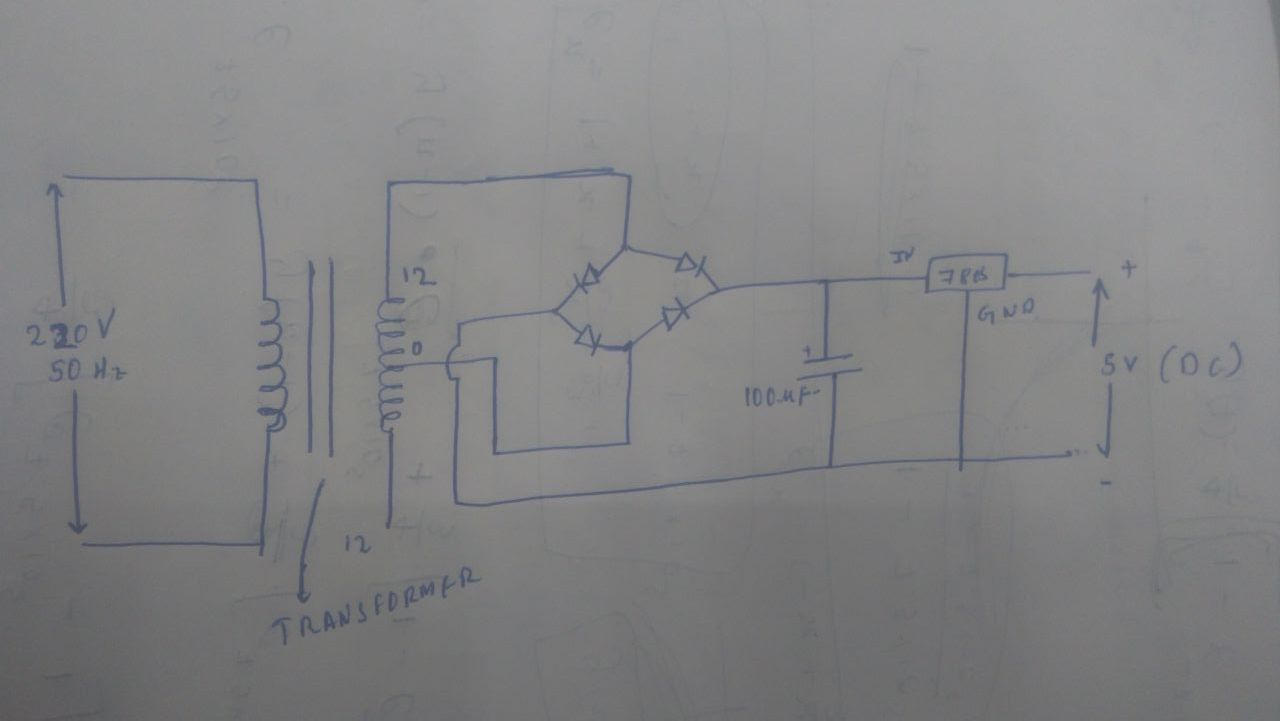
\includegraphics[width=\columnwidth]{./figs/circuit.jpg}
		\caption{Circuit diagram of a mobile charger}
		\label{fig-ckt}	
	\end{figure}
	
	\section{Circuit Explanation}
	\begin{itemize}
	\item The transformer steps down the $230 V$ AC main supply to $12 V$ AC. Note that these are RMS voltages. The peak voltage will thus be $12\sqrt{2} \approx 20V$. The transformed voltage is given by
	\begin{align}
		v(t) = 12\sqrt{2}\sin(100\pi t + \phi) V
	\end{align}
	\begin{figure}[!ht]
		\centering
		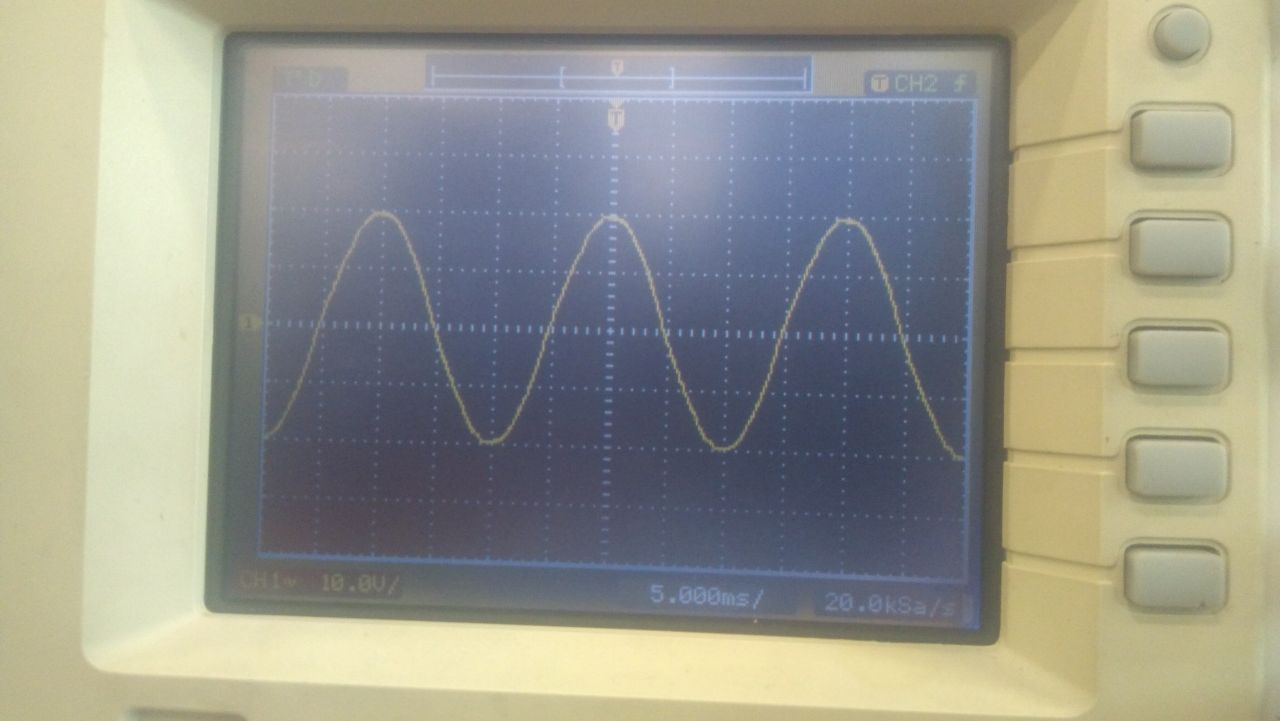
\includegraphics[width=\columnwidth]{./figs/transformer.jpg}
		\caption{CRO output after transformer}
		\label{fig-transformer}	
	\end{figure}
	
	\item The alternating current now passes through a bridge rectifier. The output is a pulsating DC wave whose peak is $12\sqrt{2}V$. The voltage at this stage is given by
	\begin{align}
		v(t) = 12\sqrt{2}\abs{\sin(100\pi t + \phi)} V
	\end{align}
	\begin{figure}[!ht]
		\centering
		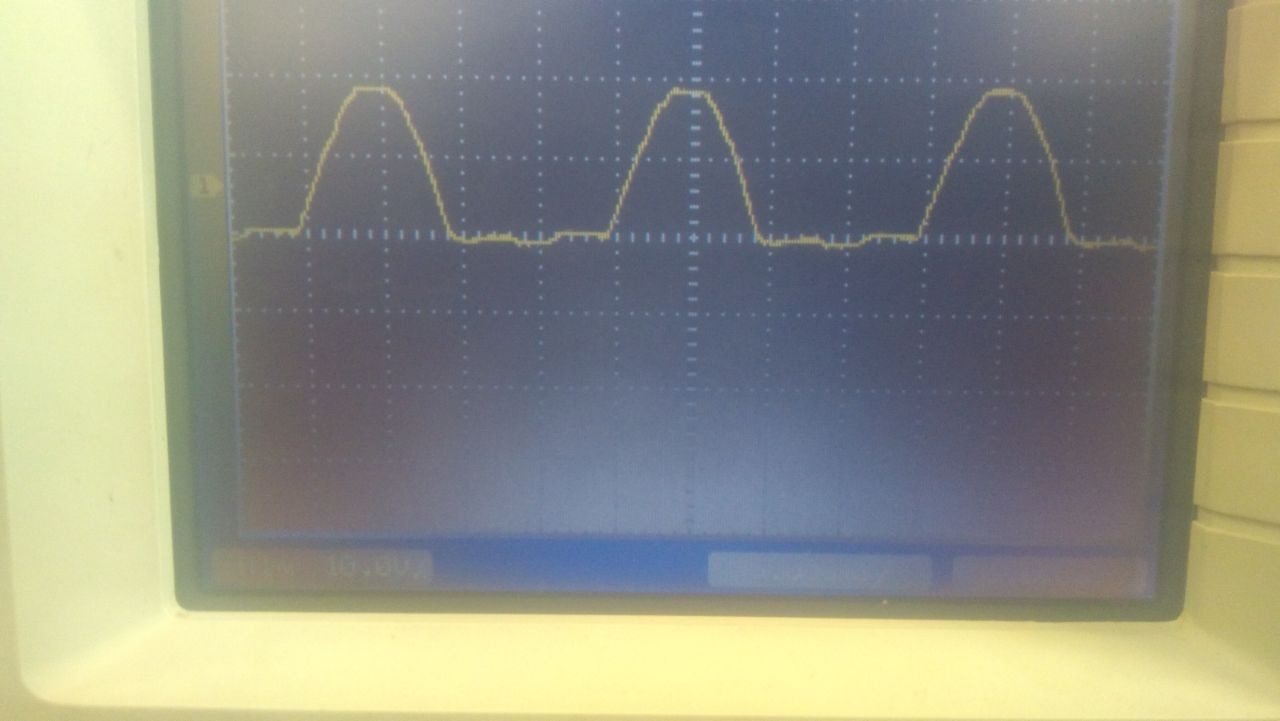
\includegraphics[width=\columnwidth]{./figs/rectifier.jpg}
		\caption{Half-wave rectified CRO outputs across a single diode}
		\label{fig-rectifier-2}	
	\end{figure}
	
	\item A capacitor is used as a low-pass filter here to choose only the zero frequency component thereby converting the current into pure DC of $12\sqrt{2}V$
	\begin{align}
		v(t) = 12\sqrt{2}V
	\end{align}
	\begin{figure}[!ht]
		\centering
		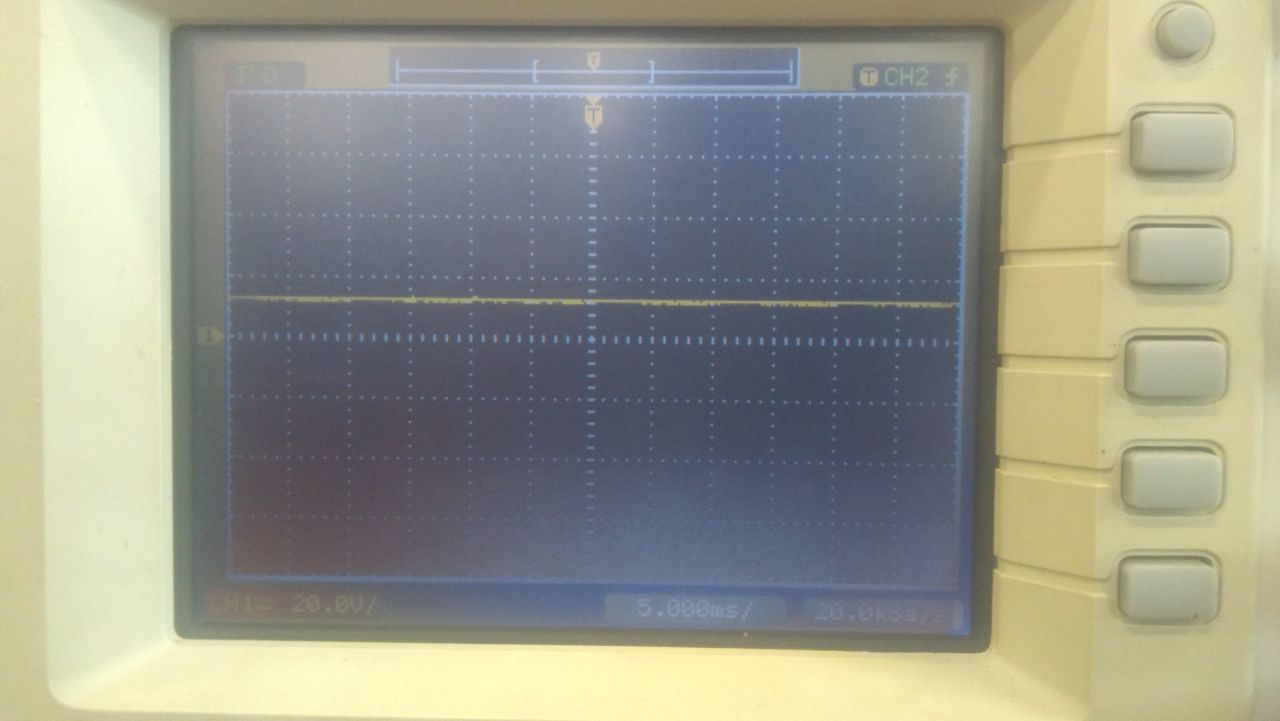
\includegraphics[width=\columnwidth]{./figs/filter.jpg}
		\caption{Filtered CRO output}
		\label{fig-filter}	
	\end{figure}
	
	\item Finally, the 7805 regulator stabilizes the output by eliminating noise and converts it into $5 V$ DC which is then used to charge the mobile phone.
	\begin{align}
		v(t) = 5 V 
	\end{align}
	\begin{figure}[!ht]
		\centering
		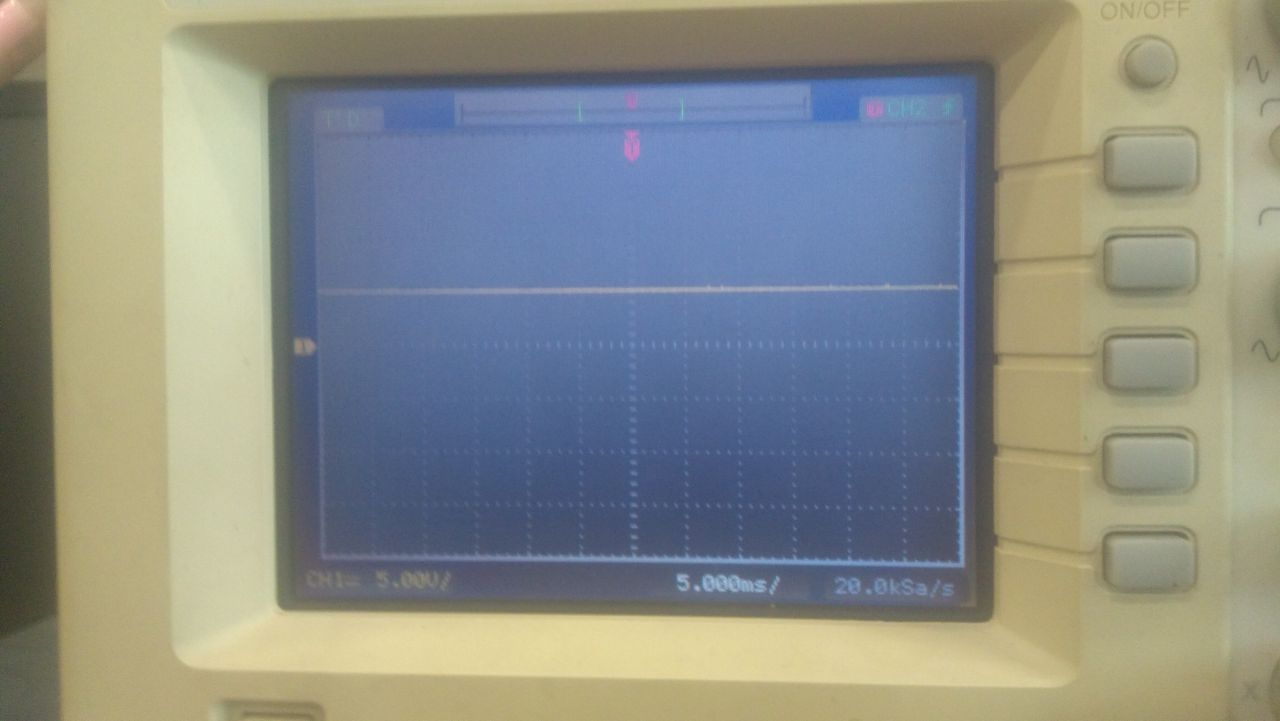
\includegraphics[width=\columnwidth]{./figs/regulator.jpg}
		\caption{Regulated CRO output}
		\label{fig-regulator}	
	\end{figure}
	\end{itemize}
	
	\section{Observations}
	Using a multimeter, we can verify that the output obtained is indeed $5 V$ DC. The same is evident on using a cathode-ray oscilloscope (CRO) too, which shows a constant $5 V$ voltage. The CRO can be used to see the waveforms at various other stages in the circuit too.
	
	\section{Result}	
	Once we have verified that we are obtaining $5 V$ DC output, we can plug in the USB cable into the output pin that is connected across the OUT and GND terminals of the regulator. On connecting the USB cable to the mobile phone and switching on the main supply to which the transformer is connected, we can see that the mobile phone is getting charged successfully.
	
	\end{document}
